The purpose of this case is to evaluate robustness, convergence properties, and
scalability of our SAP solver when compared against other existing methods.

The setup consists of an open container with a square base of size
$80~\text{cm}\times80~\text{cm}$ and $80~\text{cm}$ in height. Bodies are
dropped into this container in four different columns with the same number of
bodies each (see Fig. \ref{fig:clutter_snapshots}). Each column consists of an
arbitrary assortment of spheres of radius $5~\text{cm}$ and boxes with sides of
$10~\text{cm}$ in length. All bodies have density $1000\text{
kg}/\text{m}^3$ and therefore each sphere has a mass of approximately
$0.524\text{ kg}$ and each box has a mass of $1.0\text{ kg}$. We set a very high
contact stiffness of $k=10^{12}\text{ N}/\text{m}$ so that the model is in the
\emph{near-rigid} regime. The dissipation time scale is set to equal the time
step and the friction coefficient of all surfaces is $\mu=1.0$.
\begin{figure}[t]
    \centering
    %trim={<left> <lower> <right> <upper>}
    \adjincludegraphics[width=0.49\columnwidth,trim={0 {0.05\height} 0 0},clip]{figures/clutter/clutter_w_walls_t0.png}
    \adjincludegraphics[width=0.49\columnwidth,trim={0 {0.05\height} 0 0},clip]{figures/clutter/clutter_no_walls_t0.png}\\
    \vspace{0.1cm}
    \adjincludegraphics[width=0.49\columnwidth,trim={0 {0.05\height} 0 0},clip]{figures/clutter/clutter_w_walls_t2_zoom.png}
    \adjincludegraphics[width=0.49\columnwidth,trim={0 {0.05\height} 0 0},clip]{figures/clutter/clutter_no_walls_t2_zoom.png}
    \caption{Initial conditions (top) and an intermediate configuration after $2$ seconds of
    simulated time (bottom) for the clutter setup with (left) and without
    (right) walls. Many of the spheres in the configuration with no walls
	roll outside the frame in the intermediate configuration.}
    \label{fig:clutter_snapshots}
\end{figure}

We first run our simulations with 10 bodies per column for a total of 40 bodies.
We simulate 10 seconds using time steps of size $\delta t = 10\text{ ms}$.
Number of solver iterations and wall-clock time per time step are reported in
Fig. \ref{fig:clutter_w_walls_nb40} for the three solvers. We observe that SAP
needs to perform a larger number of iterations during the very energetic initial
transient. As the system reaches a steady state, however, SAP warm starts very
effectively, performing only about $3$ iterations per time step. Even though
SAP necessities a larger number of iterations to converge than Geodesic IPM during this initial transient, the wall-clock time per time step is very
similar. This tells us that SAP's cost per iteration is lower than that of
Geodesic IPM, even when they both use the same supernodal algebra. Unlike SAP and Geodesic IPM that benefit from warm start, we see that Gurobi performs
about $9$ iterations per time step in both the initial transient and the steady state.
\begin{figure}[!h]
	\centering
    %trim={<left> <lower> <right> <upper>}
    \adjincludegraphics[width=0.49\columnwidth,trim={0 0 0 0},clip]{figures/clutter/iterations_nb40.png}
    \adjincludegraphics[width=0.49\columnwidth,trim={0 0 0 0},clip]{figures/clutter/wall_clock_nb40.png}    
	\caption{\label{fig:clutter_w_walls_nb40} 
	Iterations and wall-clock time per time step for the clutter case with 40 bodies and with walls.}
\end{figure}

Figure \ref{fig:clutter_line_search} shows two examples of convergence history
for the case with walls. We denote with $\ell^0$ to the cost evaluated at the
initial guess, the previous time step velocity. With $\ell_*$ we denote the
optimal cost, which we approximate with its value from the last iteration. At
step 60 during the initial transient for which SAP requires 21 iterations to
converge, we observe that the algorithm reaches quadratic convergence after an
initial linear convergence transient. At step 520, past the initial energetic
transient, SAP exhibits linear convergence and satisfies the convergence
criteria within 5 iterations.
\begin{figure}[!h]
	\centering
    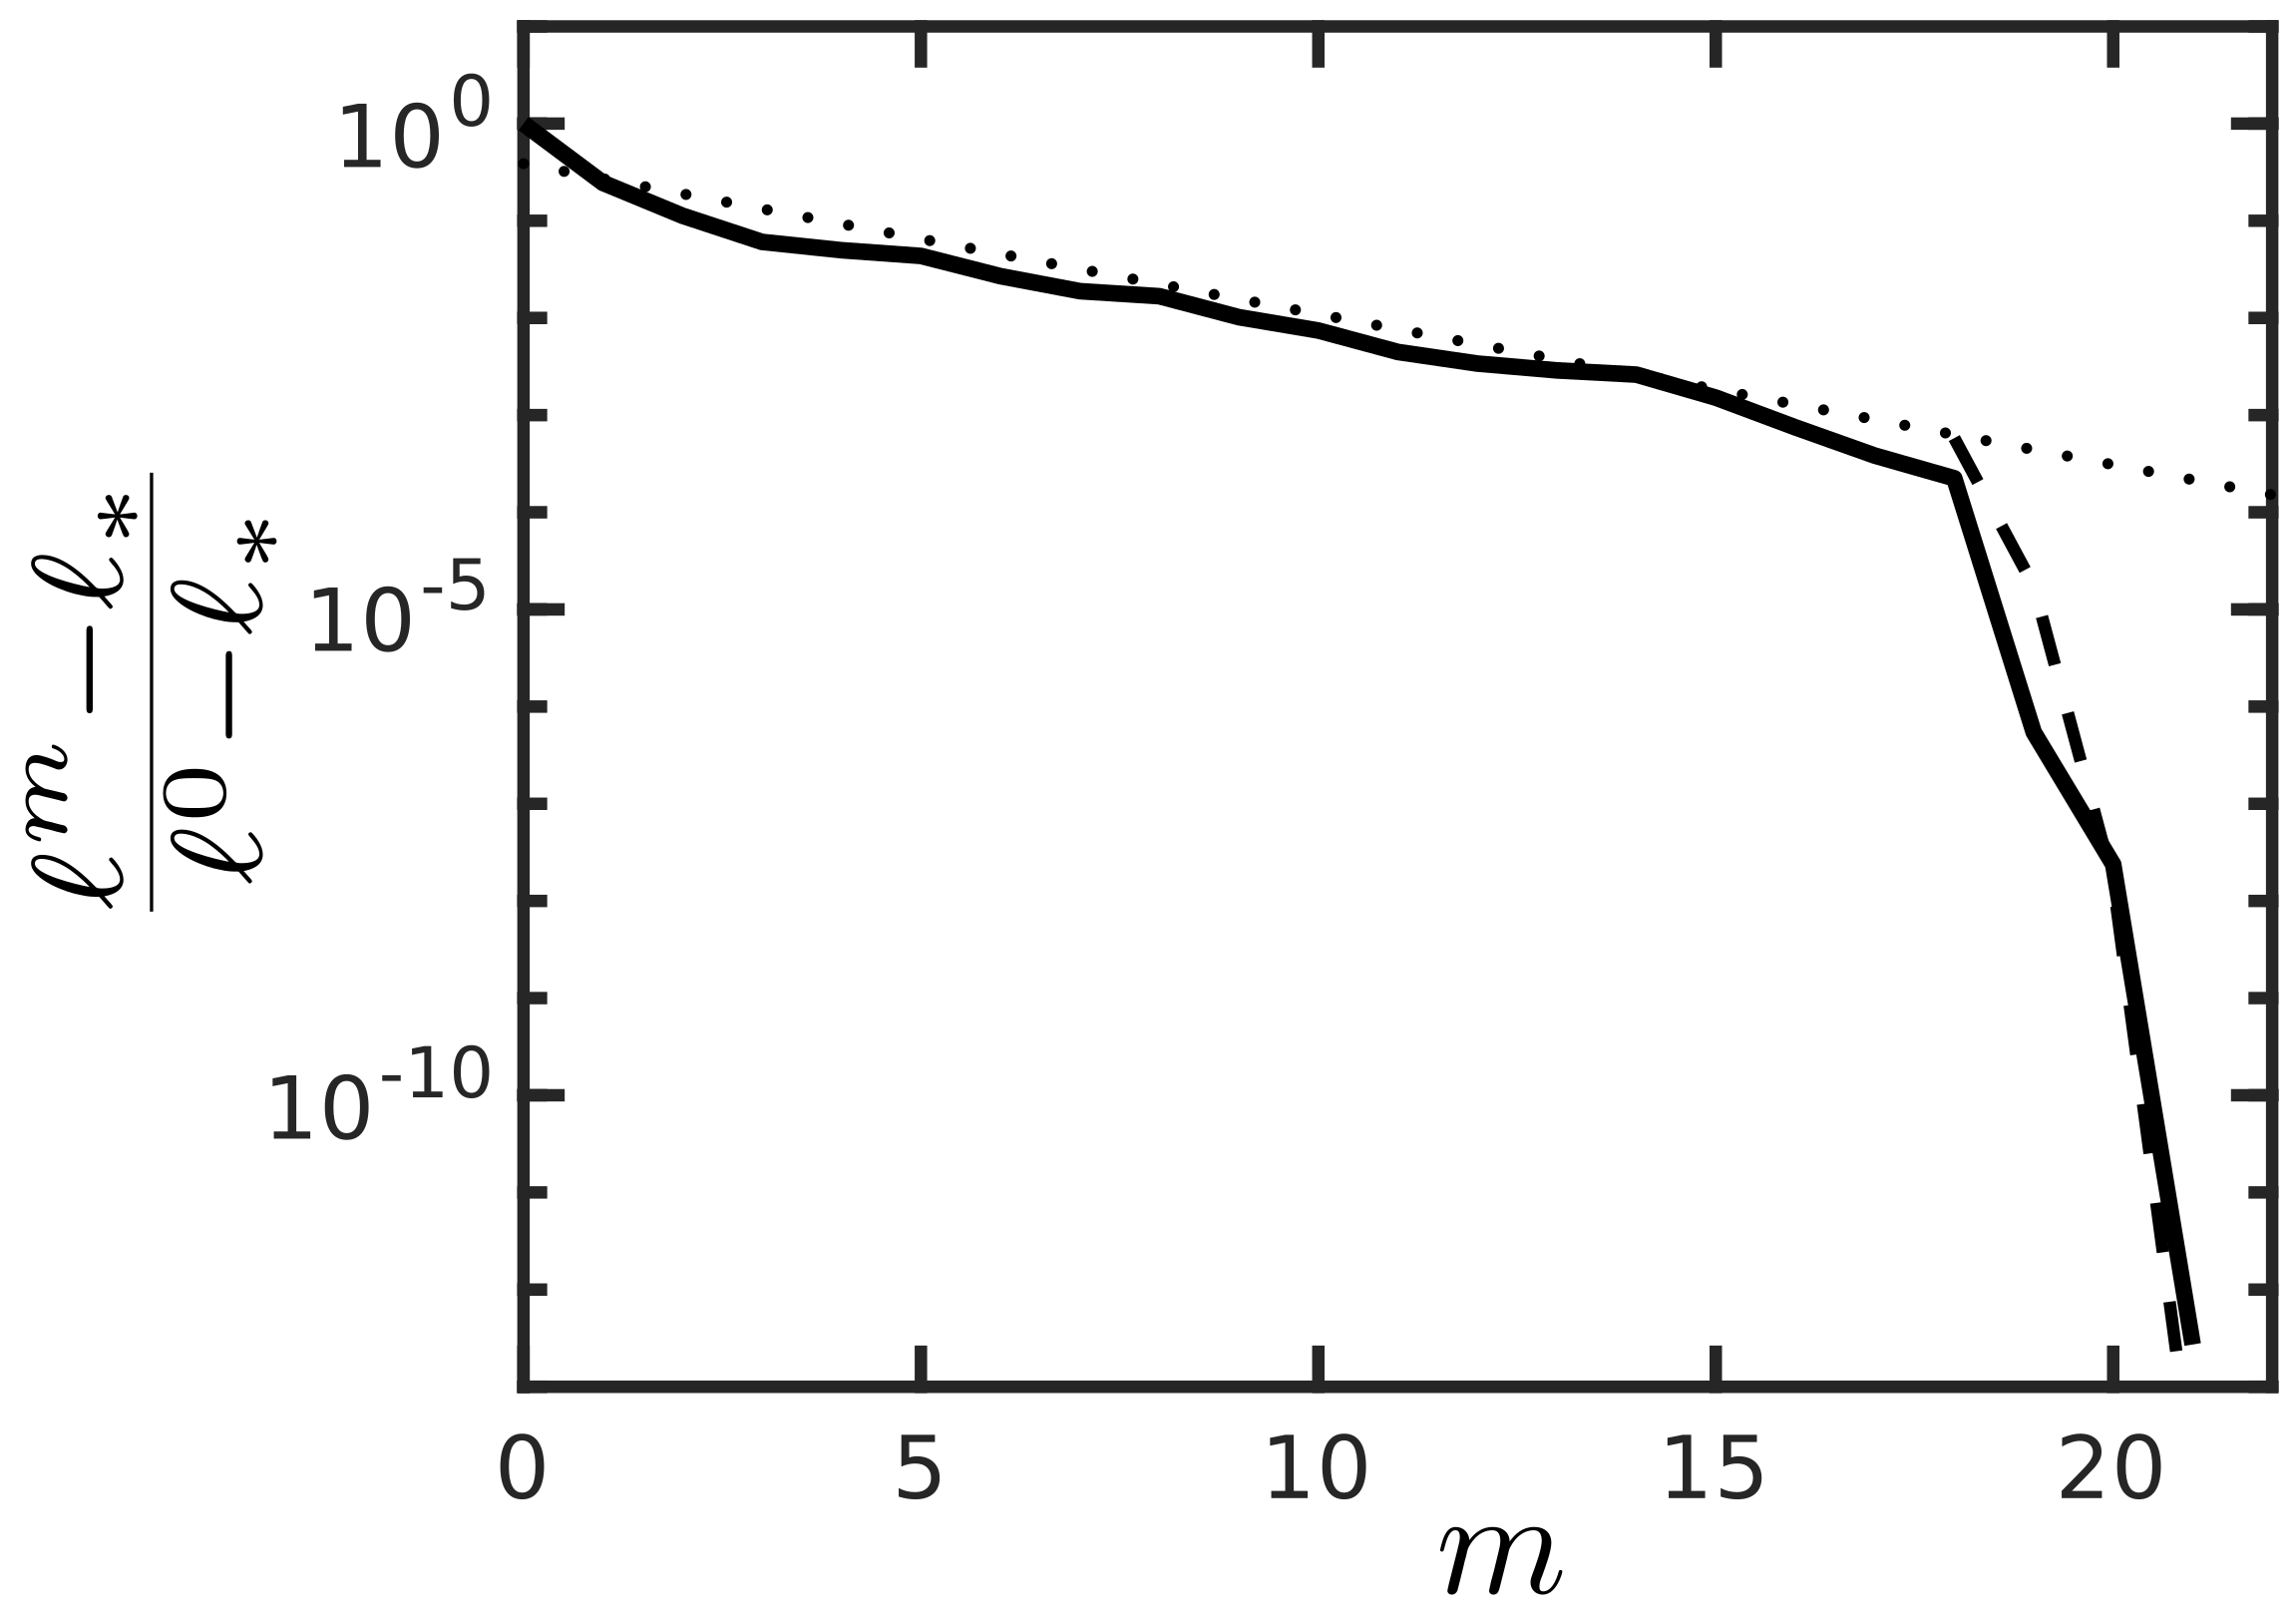
\includegraphics[height=0.34\columnwidth]{figures/clutter/normalized_cost_step60_21its_wwalls_latex_labels.png}
	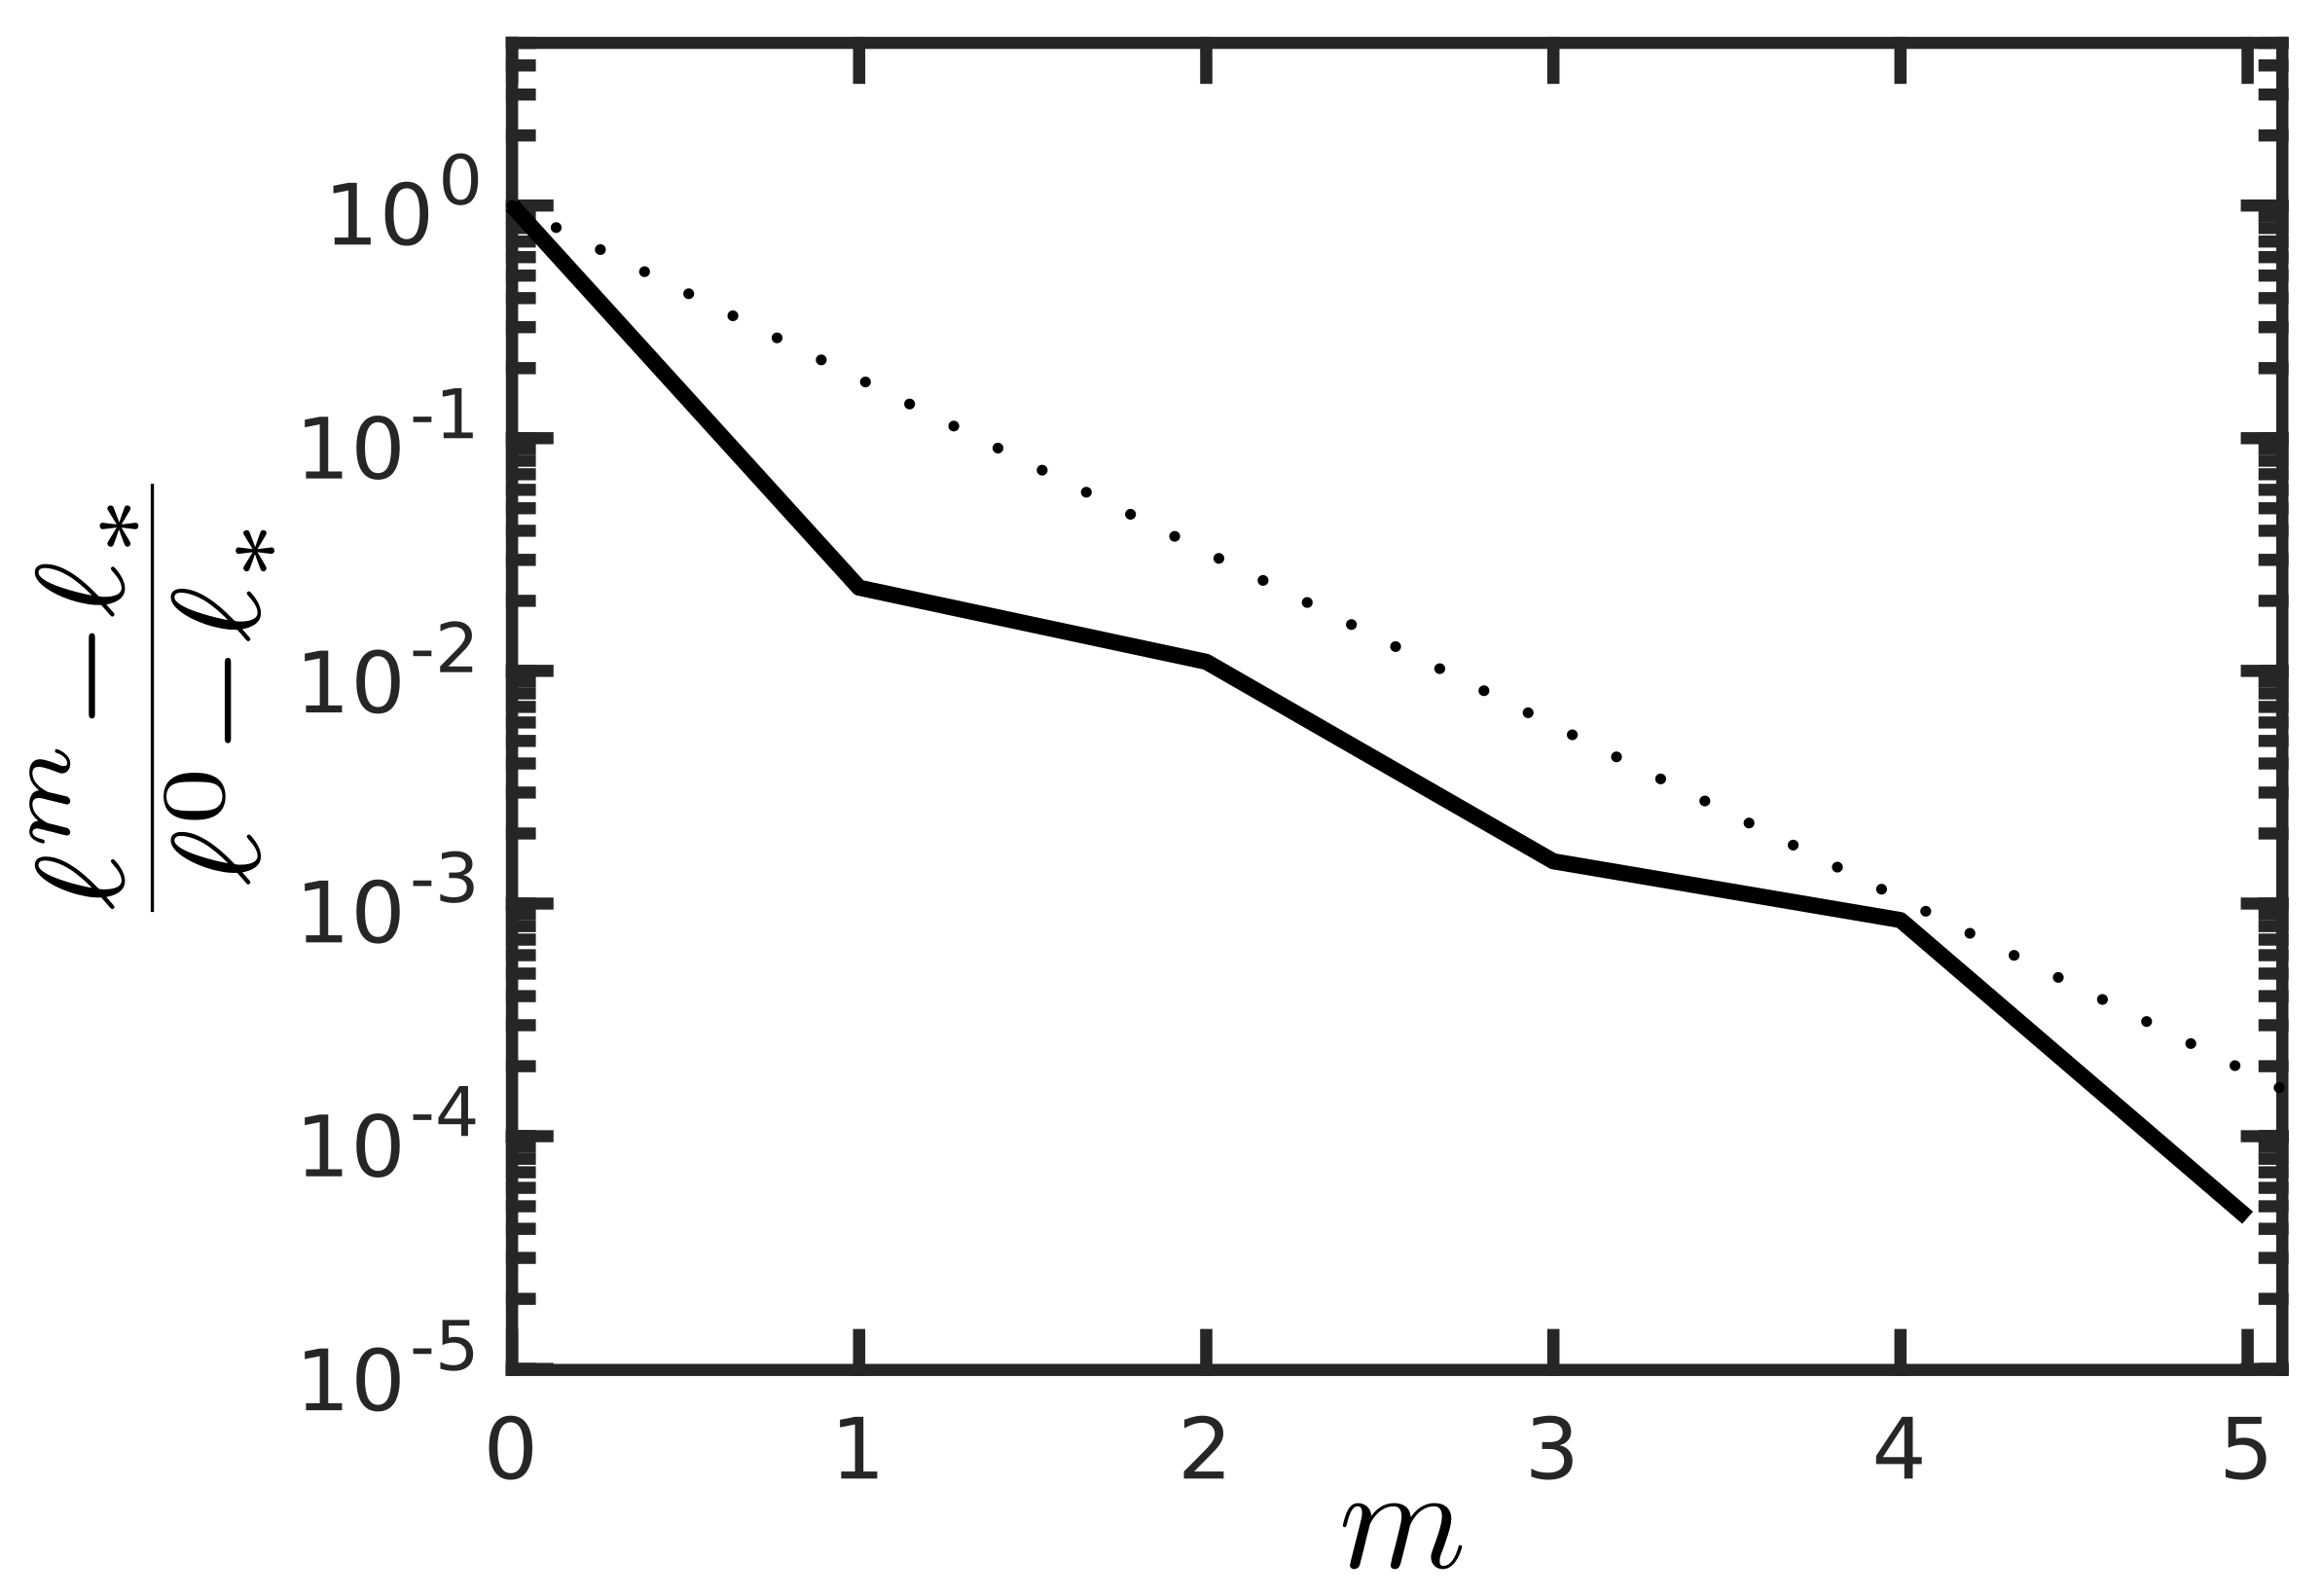
\includegraphics[height=0.34\columnwidth]{figures/clutter/normalized_cost_step520_5its_wwalls_latex_labels.png}    
	\caption{\label{fig:clutter_line_search} 
	Cost as a function of Newton iterations for step 60 (left) and for step 520 (right) using SAP. The cost decreases monotonically. Reference lines are shown for linear convergence (dotted) and quadratic convergence (dashed).}
\end{figure}

\subsubsection{Scalability}

We evaluate the performance of SAP with different problem sizes by varying the
number of objects in the clutter with all other parameters held constant. We
study scalability of the test case both with and without walls (see
Fig. \ref{fig:clutter_snapshots}) as the variation in the setup leads to very
different sequences of contact configuration. The size of the problems can be
appreciated in Fig. \ref{fig:clutter_num_contats} showing the number of contact
constraints at the end of the simulation when objects are in steady state
against the number of objects. We observe a larger number of contacts for the
configuration without walls since in this configuration many of the boxes spread
over the ground and lay flat on one of their faces, leading to a multi-contact
configuration (see Fig. \ref{fig:clutter_snapshots} for instance). Notice that
each body contributes 6 DOFs and each contact constraint contributes 3 unknowns.
Therefore, in the case with 200 bodies, the problem involves 1200 DOFs and about
2700 contact unknowns for a total of about 3000 unknowns.
\begin{figure}[!h]
	\centering
	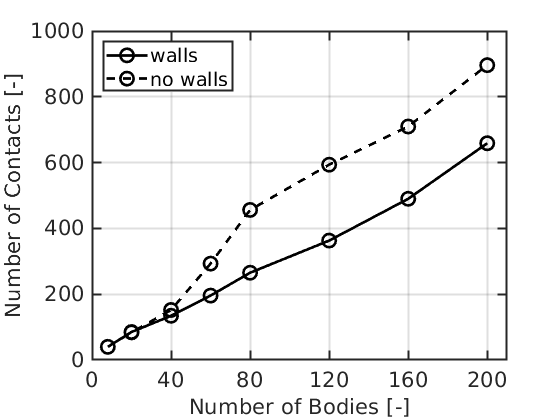
\includegraphics[width=0.7\columnwidth]{figures/clutter/number_of_contacts.png}
	\caption{\label{fig:clutter_num_contats} 
	Total number of contacts with objects in steady state at the end of the
	simulation for setups with and without walls.}
\end{figure}

We measure the total time spent by each solver and define the \emph{speedup}
against Gurobi. Figure \ref{fig:clutter_speedup} shows the speedup for both
SAP and Geodesic IPM in the configuration with and without walls.
The setup with walls is particularly difficult given that objects are
constrained to pile up, leading to a configuration in which almost all objects
are coupled with every other object by frictional contact
(see Fig. \ref{fig:clutter_snapshots}). That is, the motion of an object at the
bottom of the pile can lead to motion of another object far on top of the pile.
In contrast, the simulation with no walls leads to \emph{islands} of objects
that do not interact with each other.

In general, we observe two regimes. For problems with less than about 40 bodies,
SAP outperforms Gurobi significantly by up to a factor of 25 in the case with
walls and up to a factor of 50 with no walls. Beyond 80 bodies, Gurobi
outperforms both SAP and Geodesic IPM in the case with walls, but SAP is about
10 times faster for the case with no walls. Though SAP shows to be about twice
as fast as Geodesic IPM for most problem sizes, it can be five times faster for
small problems with 8 bodies or less.
\begin{figure}[!h]
	\centering
    %trim={<left> <lower> <right> <upper>}
    \adjincludegraphics[width=0.49\columnwidth,trim={{0.02\width} 0 {0.05\width} 0},clip]{figures/clutter/speedup_w_walls.png}
    \adjincludegraphics[width=0.49\columnwidth,trim={{0.02\width} 0 {0.05\width} 0},clip]{figures/clutter/speedup_no_walls.png}
	\caption{\label{fig:clutter_speedup} 
	Speedup against Gurobi for the configuration with walls (left) and without
	walls (right).}
\end{figure}

It could be argued that these speedup results depend on the accuracy settings of
each solver. For a fair comparison, we define the dimensionless momentum error
as
\begin{equation}
	e_m = \frac{\Vert\tilde{\nabla}\ell_p\Vert}{\max(\Vert\tilde{\mf{p}}\Vert,\Vert\tilde{\mf{j}_c}\Vert)},
	\label{eq:momentum_error}
\end{equation}
using the scaled generalized momentum quantities in Eq.
(\ref{eq:scaled_momentum_quantities}). We also define the dimensionless
complementarity slackness error as
\begin{equation}
	e_\mu = \frac{1/n_c\sum_i|\bm{g}_i\cdot\bgamma_i|}{\ell_p}.
	\label{eq:slackness_error}
\end{equation}

Figure \ref{fig:clutter_errors_w_wall} shows average values of $e_m$ and $e_\mu$
over all time steps. Since SAP satisfies the complementarity slackness exactly,
$e_\mu$ is not shown. We have verified this to be true within machine precision
for all simulated cases.

SAP's momentum error is below $10^{-5}$ as expected since this is the value used
for the termination condition. Similarly, the complementarity slackness is below
$10^{-5}$ for Geodesic IPM, since this is the value used for its own termination
condition. Gurobi does a good job at satisfying the complementarity slackness.
However, it is the solver with the largest error in the momentum equations, even
though both SAP and Geodesic IPM outperform Gurobi in most of the test cases.
These metrics demonstrate that when SAP and Geodesic IPM outperform Gurobi, it
is not at the cost of losing accuracy.
\begin{figure}[!h]
	\centering
    %trim={<left> <lower> <right> <upper>}
    \adjincludegraphics[height=0.40\columnwidth,trim={0 0 {0.05\width} 0},clip]{figures/clutter/momentum_error_w_walls.png}
	\adjincludegraphics[height=0.40\columnwidth,trim={{0.05\width} 0 {0.05\width} 0},clip]{figures/clutter/momentum_error_no_walls.png}\\
    \adjincludegraphics[height=0.40\columnwidth,trim={0 0 {0.05\width} 0},clip]{figures/clutter/optimality_condition_error_w_walls.png}
    \adjincludegraphics[height=0.40\columnwidth,trim={{0.05\width} 0 {0.05\width} 0},clip]{figures/clutter/optimality_condition_error_no_walls.png}
	\caption{\label{fig:clutter_errors_w_wall} 
	Momentum balance error $e_m$ (top) and complementarity condition error
	$e_\mu$ (bottom) for the clutter case with walls (left) and without walls
	(right).}
\end{figure}

\subsubsection{Slip Parameter}

We study the effect of the slip parameter $\sigma$ in Eq.
(\ref{eq:tangential_regularization}). As before, we use $\delta t = 10\text{ ms}$ and
simulate 40 objects for 10 seconds to a steady state configuration. At this
steady state at the end of the simulation, we compute the mean slip velocity
among all contacts. Figure \ref{fig:clutter_sigma_vt} shows this mean slip
velocity along with the estimated slip in Eq. (\ref{eq:slip_estimation}), $v_s
\approx\sigma\mu\delta t g$, shown in dashed lines. We see that the mean slip
velocity remains below the estimated slip as expected in a static configuration
with objects in stiction. In the case with walls where stiction helps to hold
the steady state static configuration, we see that the mean slip velocity
closely follows the slope of the slip estimate. Without the walls, objects do
not pile up in a complex static structure but simply lie on the ground, and
therefore, the resulting slip velocities are significantly smaller. The sudden
drop in the slip velocity for $\sigma>10^{-3}$ is caused by the sensitivity of
the final state on the value of $\sigma$. As $\sigma$ increases, so does the
slip velocity bound $v_s$ and objects in the configuration without walls can
slowly drift into a configuration leading to more contacts. In particular, boxes
are more likely to slowly drift until one of their faces lies flat
on the ground, a configuration with zero slip once steady state is reached.
Finally, we observe that when using $\sigma=10^{-3}$, the amount of slip is
negligible for robotic applications.
\begin{figure}[!h]
	\centering
	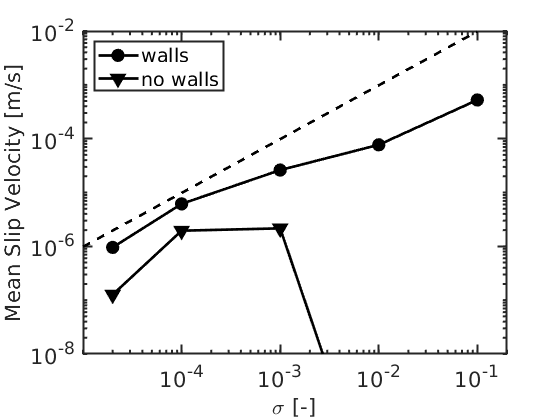
\includegraphics[width=0.7\columnwidth]{figures/clutter/sigma_vt.png}
	\caption{\label{fig:clutter_sigma_vt} 
	Mean slip velocity at the end of the simulation with objects at rest as a
	function of the slip parameter. The estimated bound $v_s = \sigma\mu\delta t g$ is shown in dashed lines.}
\end{figure}

We conclude by examining the effect of $\sigma$ on the conditioning of the
system. Figure \ref{fig:clutter_sigma} shows the condition number of the Hessian
in the final configuration and the mean number of Newton iterations throughout
the simulation. We see that the condition number scales as $\sigma^{-1}$ while
the mean number of Newton iterations is roughly proportional to  $\ln(\sigma)$.
Notice that our choice $\sigma=10^{-3}$ for this paper is placed right in the
middle, in a log scale, of the range of values examined in this study.
\begin{figure}[!h]
	\centering
    %trim={<left> <lower> <right> <upper>}
    \adjincludegraphics[width=0.49\columnwidth,trim={0 0 {0.05\width} 0},clip]{figures/clutter/sigma_iterations.png}
    \adjincludegraphics[width=0.49\columnwidth,trim={0 0 {0.05\width} 0},clip]{figures/clutter/sigma_condition_number.png}
	\caption{\label{fig:clutter_sigma} 
	Effect of the slip parameter on the mean Newton iterations per step (left) and mean condition number (right).}
\end{figure}
